\subsection{Expanded cohort}

\paragraph{Benchmark-level and paired outcomes.}
Verifier plus Jev released 428/432 legal and 130/1,008 non-execution requests, compared with 199/432 and 145/1,008 for direct DeepSeek (Fig.~\ref{fig:expansion}). In the paired comparison it gained 233 legal releases, lost four, prevented 133 false releases and introduced 118 (Table~\ref{tab:expansionpaired}). False releases rose in refunds from 20 to 42, so the Jev setup missed the prespecified benchmark-level criterion. Its equal-weight score was 0.9309, compared with 0.6584 for direct DeepSeek.

\begin{figure}[!htbp]\centering
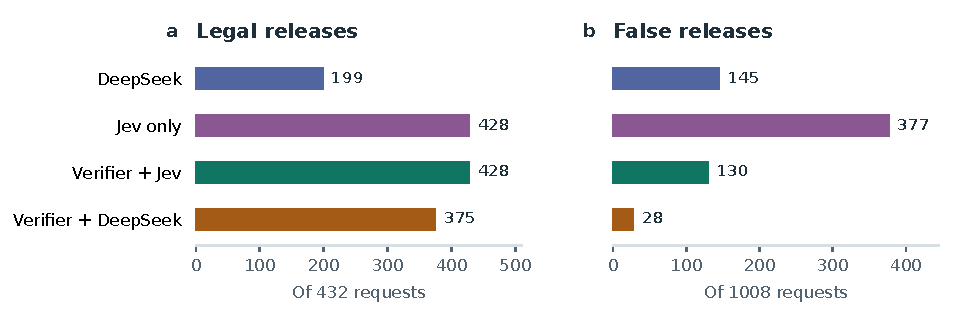
\includegraphics[width=\linewidth]{generated/effect_expansion_outcomes.pdf}
\caption{\textbf{Expanded cohort.} \textbf{a,} Legal releases out of 432. \textbf{b,} False releases out of 1,008 non-execution requests. The four policies assessed the same 1,440 proposals. The panels have separate count scales.}
\label{fig:expansion}
\end{figure}

\paragraph{Effect checks retain their contribution.}
Relative to Jev alone, the program prevented 247 false releases and preserved all 428 legal releases. The prevented cases comprise 139 per-object excesses and 108 transaction excesses. The program settled 864 requests without review, including 288 unconditional releases and 576 structured violations. The remaining 576 requests entered model review.

\begin{table}[!htbp]\centering\small
\setlength{\tabcolsep}{5pt}
\caption{Authorization and resource use for the 1,440-case expansion. Each benchmark has 144 legal and 336 non-execution cases. Score gives the equal-class probability within a benchmark or its equal-benchmark average overall. Time is mean serial API time per request, in seconds.}
\label{tab:expansionscores}
\begin{tabular}{@{}llrrrrrr@{}}\toprule
Benchmark & Method & Score & Acc.\ (\%) & Legal & False & s & CNY \\ \midrule
\tablerows{generated/effect_expansion_scores.tex}
\bottomrule\end{tabular}
\end{table}

\paragraph{Reviewer substitution changes the trade-off.}
When affirmative wording came from the wrong source, Jev accepted 129 of 144 proposals and DeepSeek accepted 28. For conditions that were actually satisfied, the Jev reviewer released 140/144 and DeepSeek released 87/144. The verifier with DeepSeek increased legal releases by 176 and reduced false releases by 117 relative to the direct control. Its false-release count decreased in every benchmark, meeting the same count criterion. Its 28 false releases included 18 cases the direct control had correctly withheld. Its equal-weight score was 0.9201. The paired difference in score between the two reviewers was 1.07 percentage points in favor of Jev (95\% family-resampling interval $-0.20$ to $2.33$).

\begin{table}[!htbp]\centering\small
\caption{Expanded-cohort paired changes for verifier plus Jev, relative to each comparator. The last column is the 95\% family-resampling interval for its score difference, in percentage points.}
\label{tab:expansionpaired}
\begin{tabular}{@{}lrrrrr@{}}\toprule
Comparator & Legal gains & Legal losses & New false & Stopped false & 95\% interval \\ \midrule
\tablerows{generated/effect_expansion_paired.tex}
\bottomrule\end{tabular}
\end{table}

The two verified policies incurred similar usage-based fees on this cohort, CNY 0.2015 with Jev and CNY 0.2000 with DeepSeek. Mean API latency was 1.701 and 0.307 seconds, respectively, with Jev's observed latency including transport retries. Across the four policies, 3,456 successful stage responses and their logged retries cost an estimated CNY 1.7148.
